\chapter{Generating Test Cases}\label{ch:tests}

\newadd{A test case is a collection of (1) input values necessary to complete some execution of the system under testing, (2) the results that must be produced after executing the test (assuming the system satisfies the intended behaviour) and (3) any inputs necessary to setup the system into the appropriate state to receive the test values~\cite{Ammann2008}.}
\newadd{Test oracles are specifications describing properties about the validity of tests cases, i.e. if the test must fail or pass. These properties may include relationships between the input given and the expected output, data validity properties, format of possible execution paths, etc. No matter the oracle format, it must be able to determine the validity of tests in a reasonable amount of time~\cite{Weyuker1982}.}

In the following, we show how to use \newadd{deterministic} occurrence graph grammars to generate test cases and oracles from (simply-typed) graph grammars that model systems. In theory, this approach can be used to generate tests for any graph grammar, since it is based only on the properties of the formalism. However, we focused on graph grammars that were generated from use cases by using the methodology presented in \cite{Junior2015}, \cite{BezerraWEIT2016} and \cite{Cota2017}.

This methodology is a systematic, computer-aided way to extract graph grammars from use cases or other text-based requirement documents. At the same time, it helps finding problems such as ambiguities, inconsistencies and omissions in the documents. Thus, providing a better specification and also an improved model. By generating tests from these grammars we are indirectly generating tests for the underlying use cases. The test generation, to be described in next sections, was implemented in Verigraph as an extension to the calculation of the occurrence graph grammars that was previously discussed.

Basically, we are interested in knowing whether each functionality of a system is truly executable \important{(why?)}, i.e. whether all the rules that represent each functionality flow are applicable.

If it happens that a functionality is not executable, we want to know exactly what is the problem that is preventing its execution. On the other hand, if it is executable, we are interested in:

\begin{enumerate}
\item the input data necessary for this functionality to execute, as well as the output data of a successful execution;

\item at least one path (for each flow) in which the rules can be applied to accomplish the functionality goals;

\item a set of constraints which can tell the test analyst how two characterize the tests into those which should pass and those which should fail;

\item a set of constraints which can tell which intermediate states of the system are valid and those that are not.
\end{enumerate}

Notice that the two first items correspond to test cases while the other two correspond to test oracles.

%First, we present a brief overview of the methodology for extracting graph grammars from use cases, after what we present the process of generating the tests cases from the extracted grammars.

\section{Overview of the extracting methodology}

Usually, use case documents consist of sets of sequential steps describing the interaction between an actor and a system in order to accomplish a specific goal. In general, one of these sets represents a successful (normal or main) execution of the system, whereas other sets represent sequences of alternative or exception flows. Moreover, use cases may also contain pre- and post-conditions used to indicate the configurations that must hold before and after their execution.

Figure~\ref{fig:tests:methodology} summarizes the methodology process proposed in \cite{Junior2015}, showing how to extract a graph grammar from a text-based requirements document. This methodology is divided into four main phases:

\begin{figure}[!ht]
  \centering
  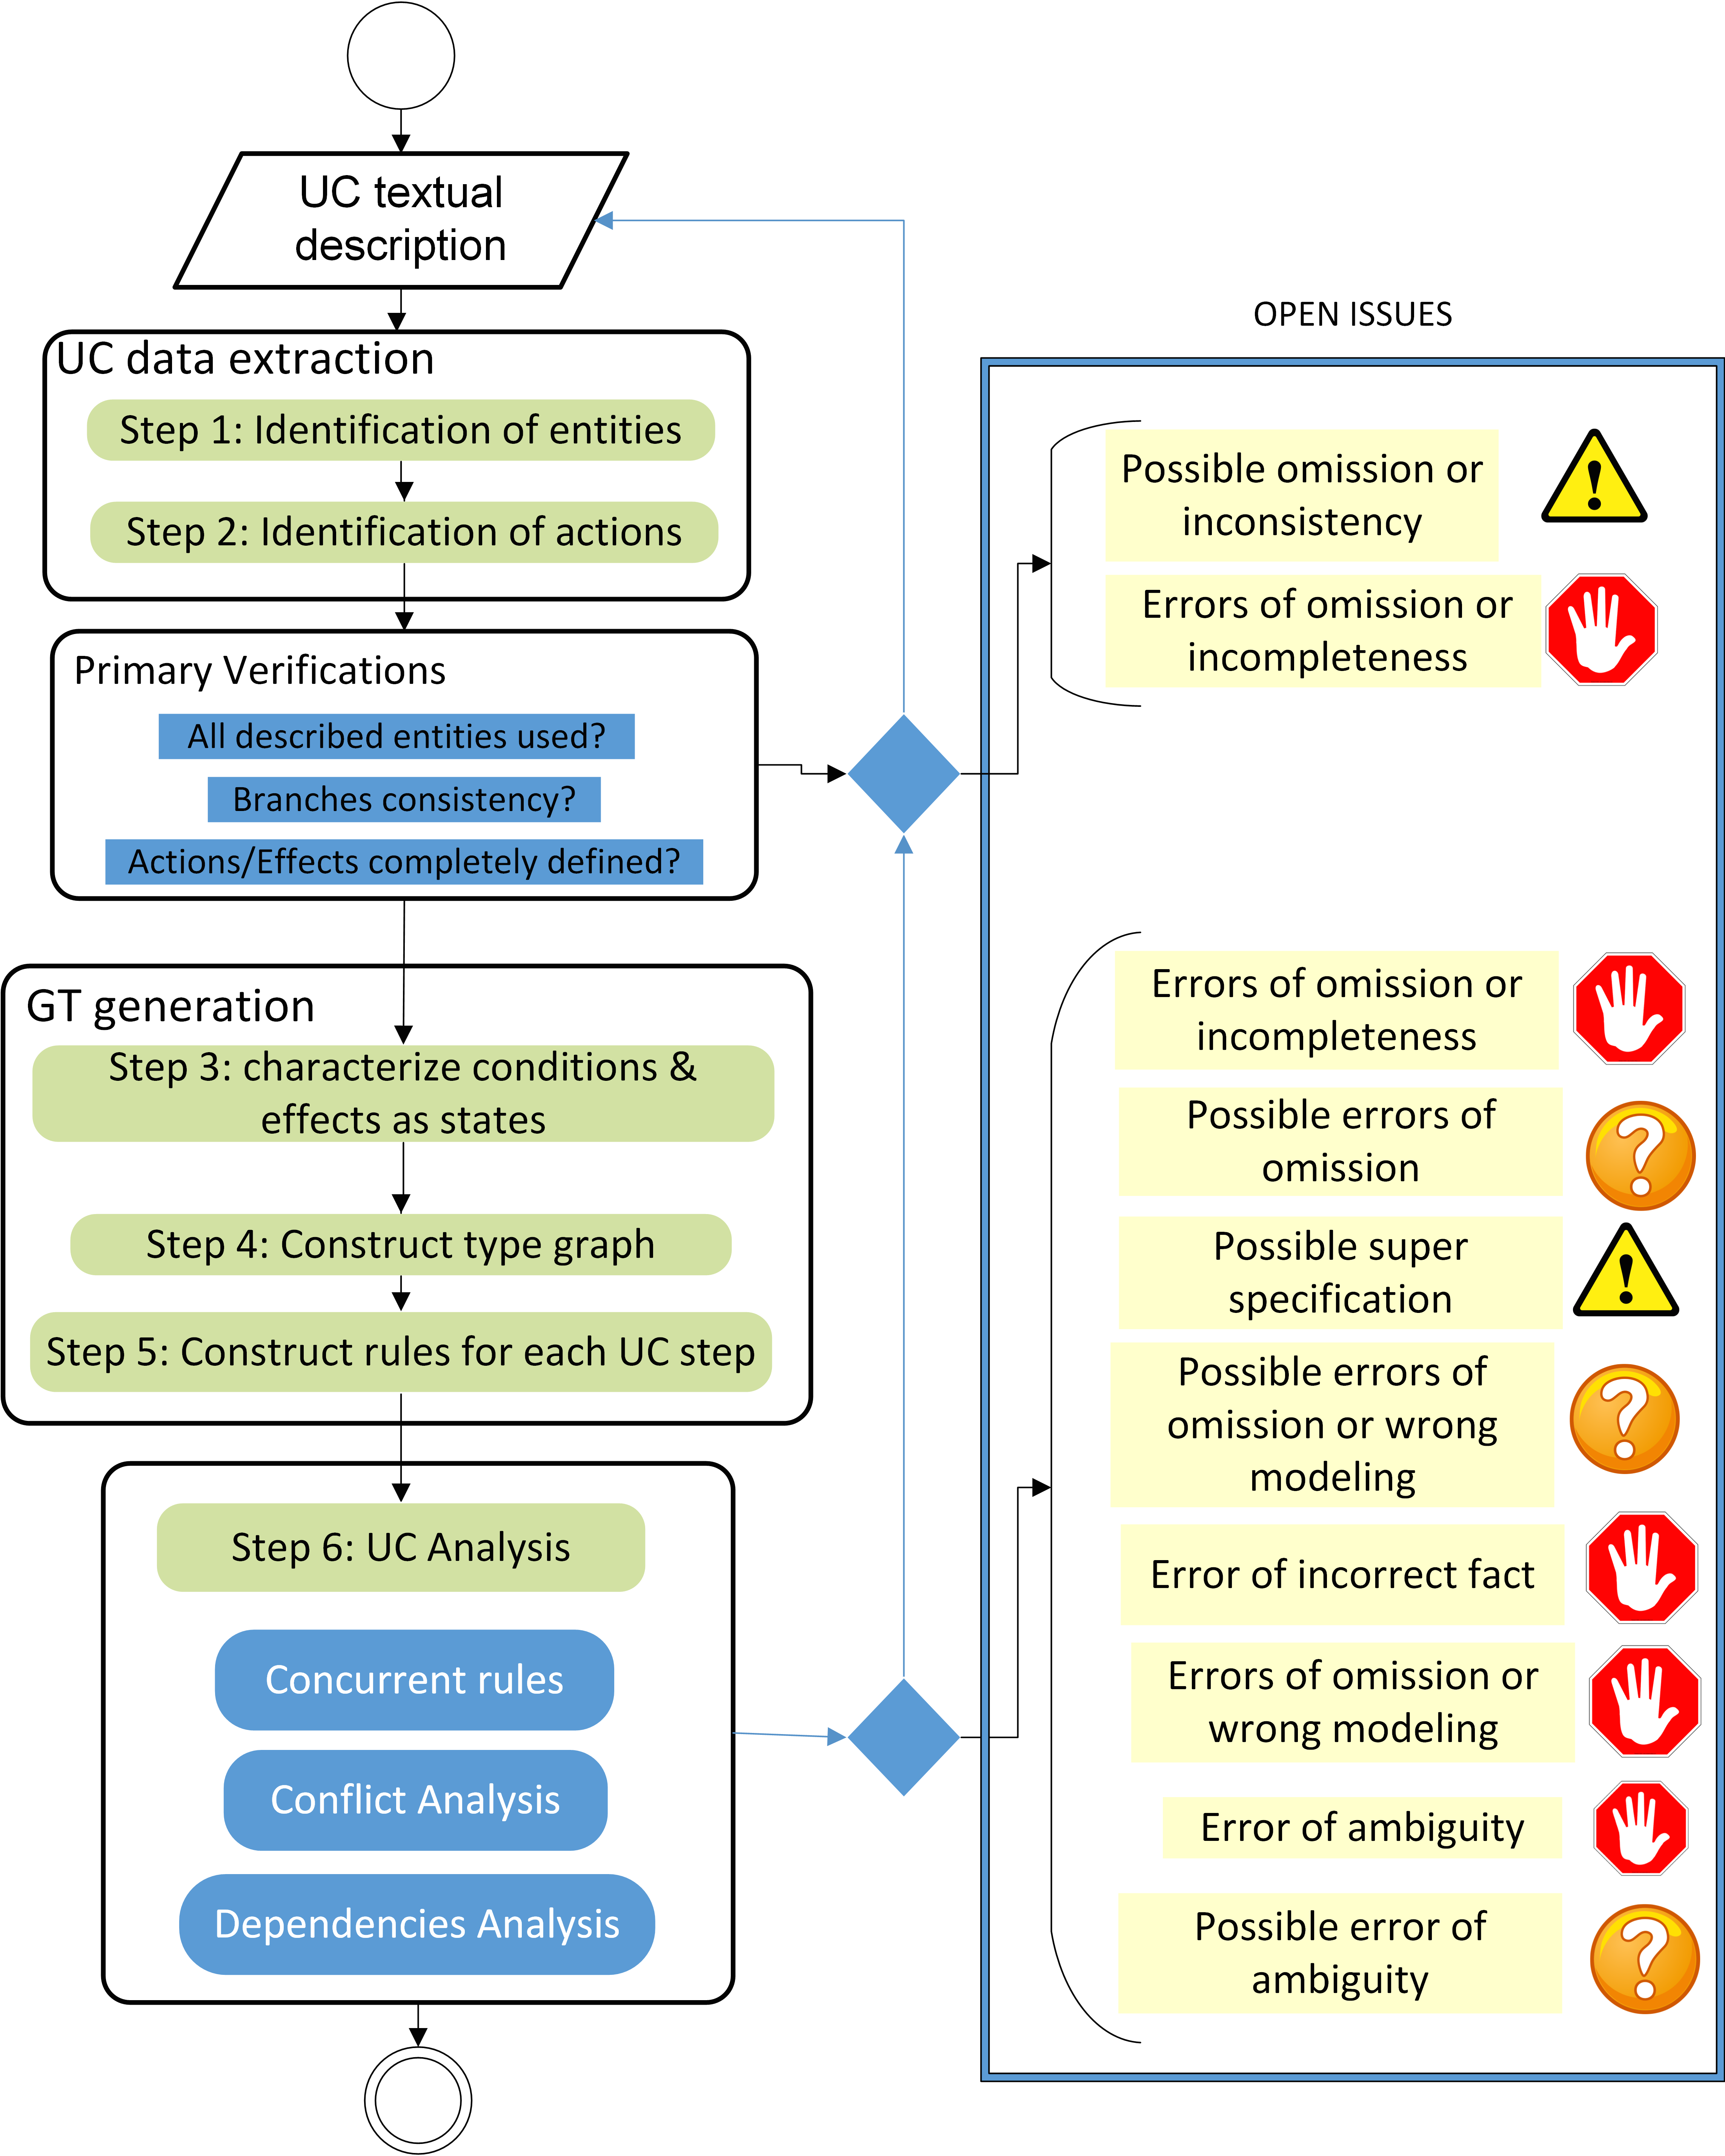
\includegraphics[scale=0.7]{images/generating-tests/methodology}
  \caption{Overview of the methodology~\cite{Junior2015}.}\label{fig:tests:methodology}
\end{figure}

\begin{description}
  \item[Data Extraction:] identification of entities and actions that will be used to construct the model.

  \item[Primary Verifications:] checking for problems that might affect or prevent the creation of the model, as well as the removal of this problems from the use case. Some examples are:entities or conditions are listed but are never used or effects of actions that are not clearly defined.

  \item[GT Generation:] construction of graph transformation model by modelling conditions and effects as graphs, building a type graph and then modelling each step of the use case as a transition rule from one state graph to another.

  \item[UC Analysis:] automated verifications over the model in order to detect possible flaws in the use case. This is step is done using verigraph and its concurrent rules, conflict and dependency analyses.
\end{description}

We use a grammar that models an e-store system in our example. This grammar was extracted, using the methodology, from a set of use cases presented in~\cite{Goins2007}. These use cases model basic e-store functionalities such as \emph{browse catalogue, user registration, login, update user information, maintain shopping cart}, among others.

Some excerpts of this grammar are shown throughout this chapter, while the complete extracted grammar can be found on appendix~\ref{app:marvel-grammar} and at the Verites repository for case studies\footnote{https://github.com/Verites/case-studies}.

\section{Generating Tests using Occurrence Graph Grammars}

\newadd{Given a graph grammar that models a system, we want to generate test cases and oracles for a complete execution of the system. By complete execution we informally mean an execution path that could be seen as an atomic operation or functionality by either a user or the system itself. For example, it could be something as simple as a successful or failing user login or something as complex as the entire process of servicing costumers, which requires attendants and waiters to be logged in, tables
to be occupied, orders to be prepared, among others.}

\newadd{\begin{definition}[Complete Execution Subset] Given a graph grammar \graphGrammar{} for a system with $n > 0$ functionalities, a \emph{complete execution subset} $F_i \subseteq P$, $\forall i \in 0\ldots n$ is a subset of the grammar rules whose application leads to achieving the goals of functionality $i$.
\end{definition}}

\begin{example} Figure~\ref{fig:tests:grammar} shows a subset of the rules from the e-store grammar. The chosen rules represent the main path of the use case \emph{browse catalogue} \important{change example and explain the goals of the functionality before showing the rules}. 

\begin{figure}[!ht]
  \centering
  \begin{subfigure}[t]{.5\textwidth}
    \centerline{\fbox{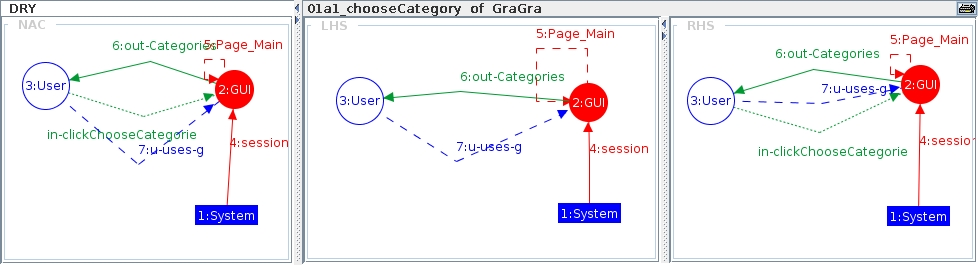
\includegraphics[scale=0.5]{images/generating-tests/grammar/rule01}}}
    \caption{Rule \emph{choose category}}
  \end{subfigure}
  \begin{subfigure}[t]{.5\textwidth}
    \centerline{\fbox{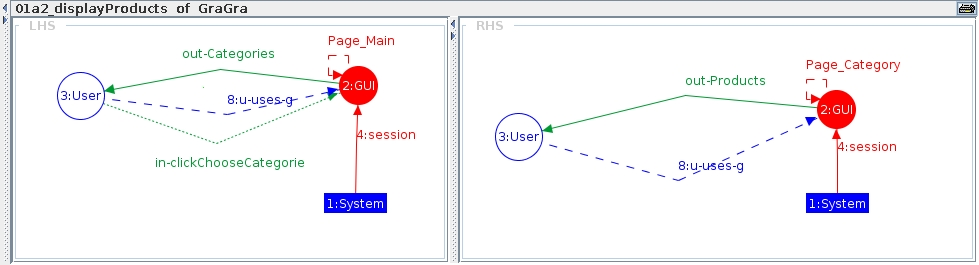
\includegraphics[scale=0.5]{images/generating-tests/grammar/rule02}}}
    \caption{Rule \emph{display products}}
  \end{subfigure}
  \begin{subfigure}[t]{.5\textwidth}
    \centerline{\fbox{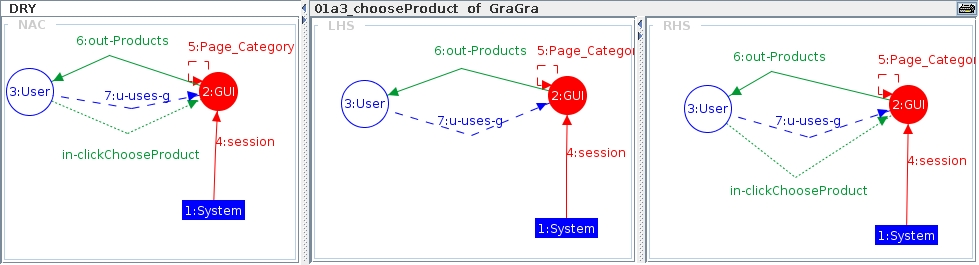
\includegraphics[scale=0.5]{images/generating-tests/grammar/rule03}}}
    \caption{Rule \emph{choose products}}
  \end{subfigure}
  \begin{subfigure}[t]{.5\textwidth}
    \centerline{\fbox{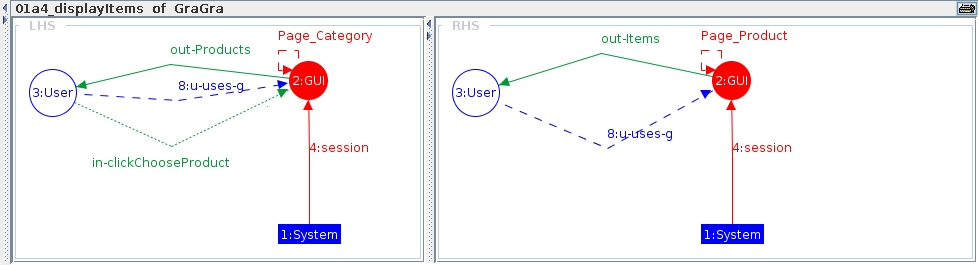
\includegraphics[scale=0.5]{images/generating-tests/grammar/rule04}}}
    \caption{Rule \emph{display items}}
  \end{subfigure}
  \caption{Rules for the use case \emph{browse catalogue}}\label{fig:tests:grammar}
\end{figure}

\begin{figure}[!ht]
\ContinuedFloat
\centering
  \begin{subfigure}[t]{.5\textwidth}
    \centerline{\fbox{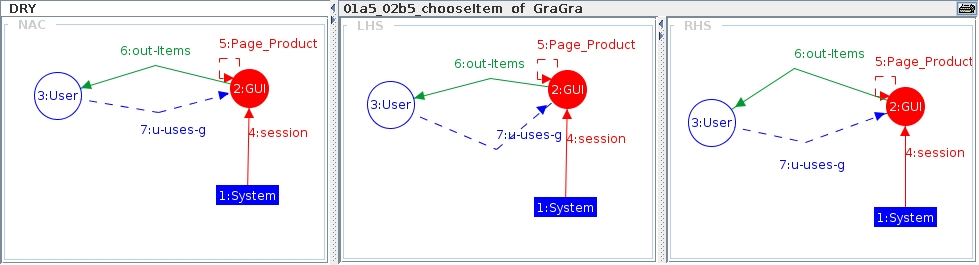
\includegraphics[scale=0.5]{images/generating-tests/grammar/rule05}}}
    \caption{Rule \emph{choose item}}
  \end{subfigure}

  \begin{subfigure}[t]{.5\textwidth}
    \centerline{\fbox{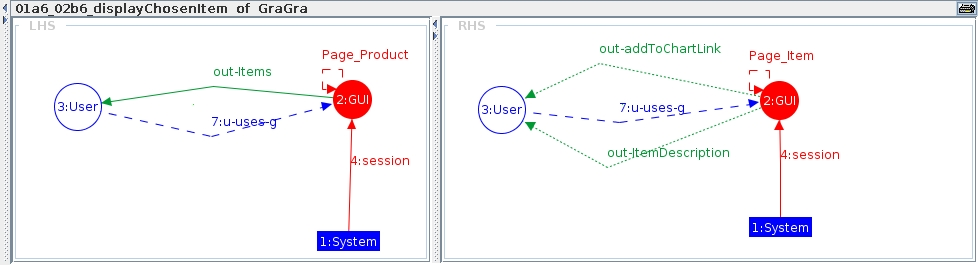
\includegraphics[scale=0.5]{images/generating-tests/grammar/rule06}}}
    \caption{Rule \emph{display chosen item}}
  \end{subfigure}
\end{figure}
\end{example}
\subsection{Preparing the input}

Along with the grammar $GG$ and its subsets of functionalities $F_i$, we will also need an \emph{input-output relation} $IO_i$ for each $F_i$, specifying the connections between the rules in the subsets. This \emph{input-output relation} identifies which elements (nodes and edges) must be the same between each pair of rules, as shown in example~\ref{ex:inout}.

\begin{definition}[Input-Output Relation] \newadd{Given a complete execution subset $F_i$, its underlying \emph{input-output relation} $IO_i$ is a set of typed-graph morphism spans of the form \mbox{$\left(R_x \leftarrow IO \rightarrow L_y\right)$} each of which connects two distinct rules $x,y \in F_i$.}

  \newadd{  The $IO$ object of each span is similar to the gluing graph of a rule, but instead of identifying the elements that are preserved by one rule, it identifies the elements that are necessarily the same between two different rules.}
\end{definition}

\important{review}  We choose the main flow of our example grammar to show how to build the $IO$ relation. First of all, the complete execution subset for this functionality is $F_1 = \{$ chooseCategory, displayProducts, chooseProduct, displayItems, chooseItem, displayChosenItem $\}$. Once having the sets of rules, we build the input-output relations for each one of them.

\begin{example}[Input-Output Relations]\label{ex:inout} \important{review} An input-output relation for a complete execution subset has the appearance of the diagram bellow, where there are several $IO$ objects connecting the right-hand side of a rule with the left-hand side of another.

    Figure~\ref{fig:tests:inout} shows how an $IO$ object connects two different rules, which is similar to how the interface graph of a rule identifies the elements that are the same in its left and right sides.

\diagram{
  & & & & IO_6\ar@{-->}[dddrrrr]\ar@{-->}[dddllll] & & & &\\
  & IO_3\ar@{-->}[ddl]\ar@{-->}[ddrrrr] & & & & & & IO_4\ar@{-->}[ddr]\ar@{-->}[ddllll] &\\
  & & IO_1\ar@{-->}[d]\ar@{-->}[dr] & & IO_5\ar@{-->}[drr]\ar@{-->}[dll] & & IO_2\ar@{-->}[d]\ar@{-->}[dl] & &\\
  L_1 & K_1\ar[l]\ar[r] & R_1 & L_2 & K_2\ar[l]\ar[r] & R_2 & L_3 & K_3\ar[l]\ar[r] & R_3\\
  }\hfill\break

  For most cases, it will not be necessary to create an $IO$ object for each pair of rules, as the $IO$ relation has some sort of transitivity. Thus, we can focus on build only a subset of it.

  Take for example the \emph{system} node in the grammar. This node should be the same along all rules, and it appears in left and right sides of all rules. Given two rules $p_1$ and $p_2$, we have the options of building the $IO$ object that identifies the system node as $L_1 \leftarrow IO \rightarrow R_2$ or $L_2 \leftarrow IO \rightarrow R_1$. Both of them having the same effect. \important{review example}

\begin{figure}[!ht]
  \centering
  \fbox{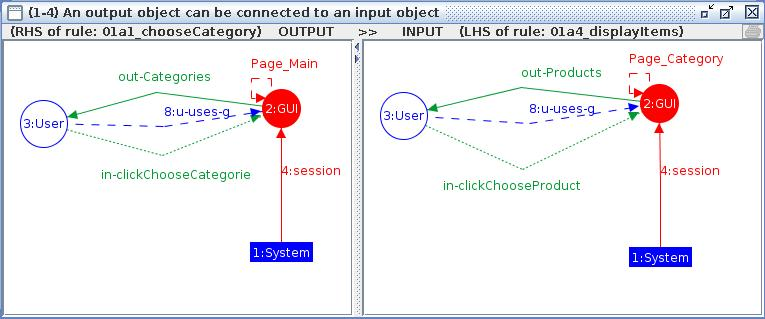
\includegraphics[scale=0.7]{images/generating-tests/grammar/inout}}
  \caption{Input-Output relation building}\label{fig:tests:inout}
\end{figure}

\end{example}

\subsection{Processing the input grammar}

\important{Explain this better, also extract it to a definition}

\newadd{Having a graph grammar \graphGrammar{} modelling a system with \mbox{$n > 0$} functionalities, the generation of test cases and oracles for each functionality $i$ is accomplished by the construction of a deterministic occurrence graph grammar $OGG_i$ using $F_i$ and $IO_i$. The construction steps are specified in Definition~\ref{def:ogg-construction}.}.

\begin{definition}[Deterministic Occurrence Graph Grammar Construction]\label{def:ogg-construction} Let \graphGrammar{} be a graph grammar, $F_i$ and $IO_i$

\begin{enumerate}
\item calculate the amalgamation (colimit) $Occ_i$ of the rules in $F_i$ with respect to $IO_i$.

\diagram{
  & & & & IO_6\ar[dddrrrr]\ar[dddllll] & & & & &\ldots\\
    & IO_3\ar[ddl]\ar[ddrrrr] & & & & & & IO_4\ar[ddr]\ar[ddllll] & & \ldots\\
    & & IO_1\ar[d]\ar[dr] & & IO_5\ar[drr]\ar[dll] & & IO_2\ar[d]\ar[dl] & & &\ldots\\
    L_1\ar[dddrrrr] & K_1\ar[l]\ar[r] & R_1\ar[dddrr] & L_2\ar[dddr] & K_2\ar[l]\ar[r] & R_2\ar[dddl] & L_3\ar[dddll] & K_3\ar[l]\ar[r] & R_3\ar[dddllll] & \ldots\ar[dddlllll]\\
    & & & & & & & & &\\
    & & & & & & & & &\\
    & & & & Occ & & & & &
}\hfill\break

\item retype the rules $F_i$ over $Occ_i$, generating a set $F'_i$ of doubly-typed graph rules.

\item calculate the occurrence relation $\leq_{occ}$ using the doubly-typed graph rules in $F'_i$.
\item calculate the set $R_i$ of restrictions over the ordering of rules applicability.
\item generate the initial and final graphs $I_i$ and $J_i$ by deleting from $Occ_i$ the elements that are created (resp. deleted) by the rules in $F'_i$ according to existential relation.
\item find one or more total orderings that respect the occurrence relation and restrictions.
%\item one or more total orderings that do not respect the relations or restrictions
\end{enumerate}

  The Occurrence Graph Grammar representing execution of the functionality $i$ is given by $OGG_i = (Occ_i, I_i,F_i)$, iff $OGG_i$ respects the conditions imposed by Definition~\ref{def:ogg}.
\end{definition}

In the first step of the construction, the amalgamation of the rules in $F_i$ w.r.t. $IO_i$ is responsible to ``glue'' the graphs of all rules in one single graph $Occ_i$, while identifying the items that are meant to be the same element at the grammar execution. %%The colimit of a diagram such as the one presented in Example~\ref{ex:inout} has the following format, where $Occ$ is the amalgamation object, i.e. $Occ$ contains all the concrete elements of the rules where it came from:
If $Occ_i$ is a \emph{core graph} according to definition~\ref{def:core-graph}, we can create a doubly-typed graph grammar $OGG_i$ that is also a strongly-safe grammar and therefore a candidate to be an occurrence graph grammar.

Remember that, if there is more than one rule that deletes or creates the same element, it is not possible to apply all rules of this functionality, and $OGG_i$ can not be a deterministic occurrence graph grammar.

\begin{example}[Amalgamation example]\label{ex:amalgamation} Figure~\ref{fig:tests:colimit} shows the object resultant from the amalgamation of the rules presented in Figure~\ref{fig:tests:grammar}.

\begin{figure}[!ht]
  \centering
  \fbox{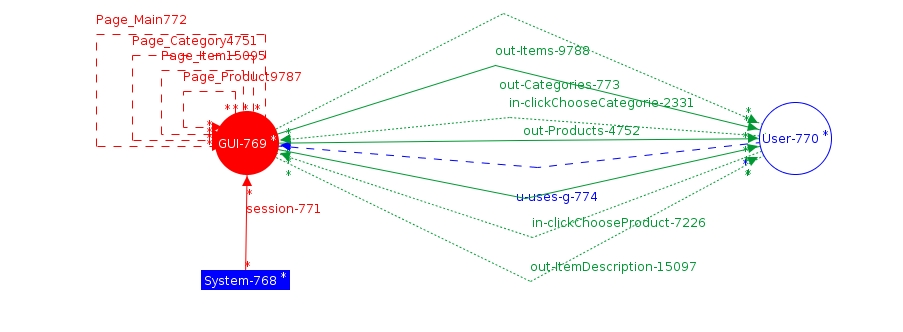
\includegraphics[scale=0.4]{images/generating-tests/colimit}}
  \caption{Amalgamation (colimit) of rules according to the IO relation.}\label{fig:tests:colimit}
\end{figure}

\end{example}

After identifying that $OGG_i$ is in fact a strongly-safe graph grammar, we can extract the initial and final graphs of $OGG_i$ by removing from the core graph the created and deleted elements, respectively. If they are valid graphs, we have the input and output data for the test case. Otherwise, if they have dangling edges, it is not possible to apply all rules of the functionality, since it would begin in or lead to an inconsistent state.

\begin{example}[Initial and Final Graphs Example] Figure~\ref{fig:tests:graphs} shows the initial and final states for the main flow of \emph{browse catalogue}.

\begin{figure}[!ht]
  \centering
  \begin{subfigure}[t]{.5\textwidth}
    \centerline{\fbox{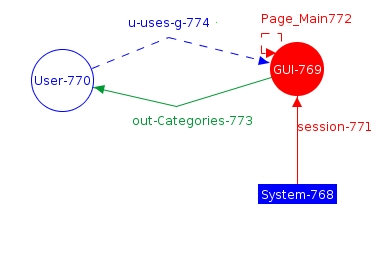
\includegraphics[scale=0.5]{images/generating-tests/grammar/initial}}}
    \caption{Initial graph}
  \end{subfigure}%
  \begin{subfigure}[t]{.5\textwidth}
    \centerline{\fbox{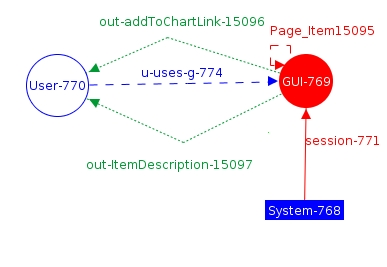
\includegraphics[scale=0.5]{images/generating-tests/grammar/final}}}
    \caption{Final graph}
  \end{subfigure}
  \caption{Instance graphs}\label{fig:tests:graphs}
\end{figure}
\end{example}

\subsection{Analysing results}

Once the previous verifications were successful, we can build the occurrence relation (and any other relation discussed on chapter~\ref{ch:process}) to verify if $OGG_i$ can really be an occurrence graph grammar. If no abstract dependencies or conflicts are found, then the concrete relations are sufficient to do this verification, thus we simply need to check if there is a total ordering compatible with the relations.

\begin{example}[Occurence Relation] Figure~\ref{fig:tests:relation} shows the relation between the rules of this occurrence graph grammar.
\end{example}

If the set $R$ of \emph{occurrence relation restrictions} is not empty, we also need to check if there is a total ordering of the occurrence relation that respects these restrictions.

As this seems to be a hard problem, in the complexity sense, we left this last implementation as a future work. However, we still use the restrictions to generate a set of tests regarding the consistency of the system states.

In our case studies, no such situation was found. We believe that it happens because we used grammars extracted from real use cases, where usually there are (possibly many) sequential connections between the actions, which forces the rules to be connected via the \emph{occurrence relation} and avoids abstract restrictions.

The output of verigraph for test case generation is shown on Figures~\ref{fig:tests:checklist} and~\ref{fig:tests:relation}. On the first figure, verigraph performs the basic verifications to check whether the generated output is, in fact, an occurrence grammar.

\begin{figure}[!ht]
\caption{Tool command line output}
\begin{minted}[linenos=true, breaklines,fontsize=\small]{shell}
Testing Serialization:
[OK] Unique creations and deletions
[OK] Initial graph is valid
[OK] Final graph is valid
[OK] Concrete occurrence relation is a total order
[OK] Concrete elements relation is a total order
[OK] There are no abstract restrictions
Analysis written in tmp/output_analysis
Test cases written in tmp/output_test_cases
Saved in tmp/output.ggx
\end{minted}
  \label{fig:tests:checklist}
\end{figure}

\begin{figure}[!ht]
\caption{Output for browse catalogue main flow}
\begin{minted}[linenos=true, breaklines,fontsize=\small]{ruby}
Rules involved: {
["01a1_chooseCategory", "01a2_displayProducts", "01a3_chooseProduct", "01a4_displayItems", "01a5_02b5_chooseItem", "01a6_02b6_displayChosenItem"]
}

Concrete Rules Relation: {
[("01a1_chooseCategory" < "01a2_displayProducts"), ("01a1_chooseCategory" < "01a3_chooseProduct"), ("01a1_chooseCategory" < "01a4_displayItems"), ("01a1_chooseCategory" < "01a5_02b5_chooseItem"), ("01a1_chooseCategory" < "01a6_02b6_displayChosenItem"),...]
}

Elements involved: {
[Node 768,Node 769,Node 770,Edge 771,Edge 772,Edge 773,Edge 774,Edge 2331,Edge 4751,Edge 4752,Edge 7226,Edge 9787,Edge 9788,Edge 15095,Edge 15096,Edge 15097]
}

Elements Relation: {
[(Edge 772 < Edge 4751),(Edge 772 < Edge 4752),(Edge 772 < Edge 7226),(Edge 772 < Edge 9787),(Edge 772 < Edge 9788),(Edge 772 < Edge 15095),(Edge 772 < Edge 15096),(Edge 772 < Edge 15097),(Edge 773 < Edge 4751),(Edge 773 < Edge 4752),(Edge 773 < Edge 7226) ...]
}

Rules Ordering: {
["01a1_chooseCategory","01a2_displayProducts","01a3_chooseProduct", "01a4_displayItems","01a5_02b5_chooseItem", "01a6_02b6_displayChosenItem"]
}

Element Ordering: {
[Node 768,Node 769,Node 770,Edge 771,Edge 772,Edge 773,Edge 774,Edge 2331,Edge 4751,Edge 4752,Edge 7226,Edge 9787,Edge 9788,Edge 15095,Edge 15096,Edge 15097]
}

Set of Abstract Restrictions: {
[]
}
\end{minted}
  \label{fig:tests:relation}
\end{figure}
The analysis file contains the results for calculation of conflicts and dependencies among rules and among elements. The test cases file contains the information relevant to test designer.
The \code{.ggx} presents the occurrence graph grammar constructed, together with its initial and final graphs.

The test oracles are represented by the concrete rules relation and the set of abstract restrictions: any path that complains to the format imposed by them is considered valid and must always succeed. On the other hand, paths that break at least one of such restrictions are considered invalid, and their tests must always capture them as failures.

The tests are represented by the rules and element ordering and also by the initial and final graphs. The ordering of rules is one of (possibly) many valid orders in which the rules can be applied.

The ordering of elements represent an ordering in which the state of the system may be constructed. While the initial and final graphs translate the valid formats for the input and output of each test.

More specific usability details can be found on the Verigraph tutorial, whose current version is presented on appendix~\ref{app:tutorial}.

\important{\section{Tests Validity}}


